% System design of counterparty co-commitment (compiled to F1_design.pdf; included by main.tex)
\documentclass[tikz,border=3pt]{standalone}
\usepackage{amsmath,amssymb}
\usetikzlibrary{positioning,arrows.meta,fit,backgrounds,calc}
\newcommand{\Sk}{\mathsf{Sk}}
\begin{document}
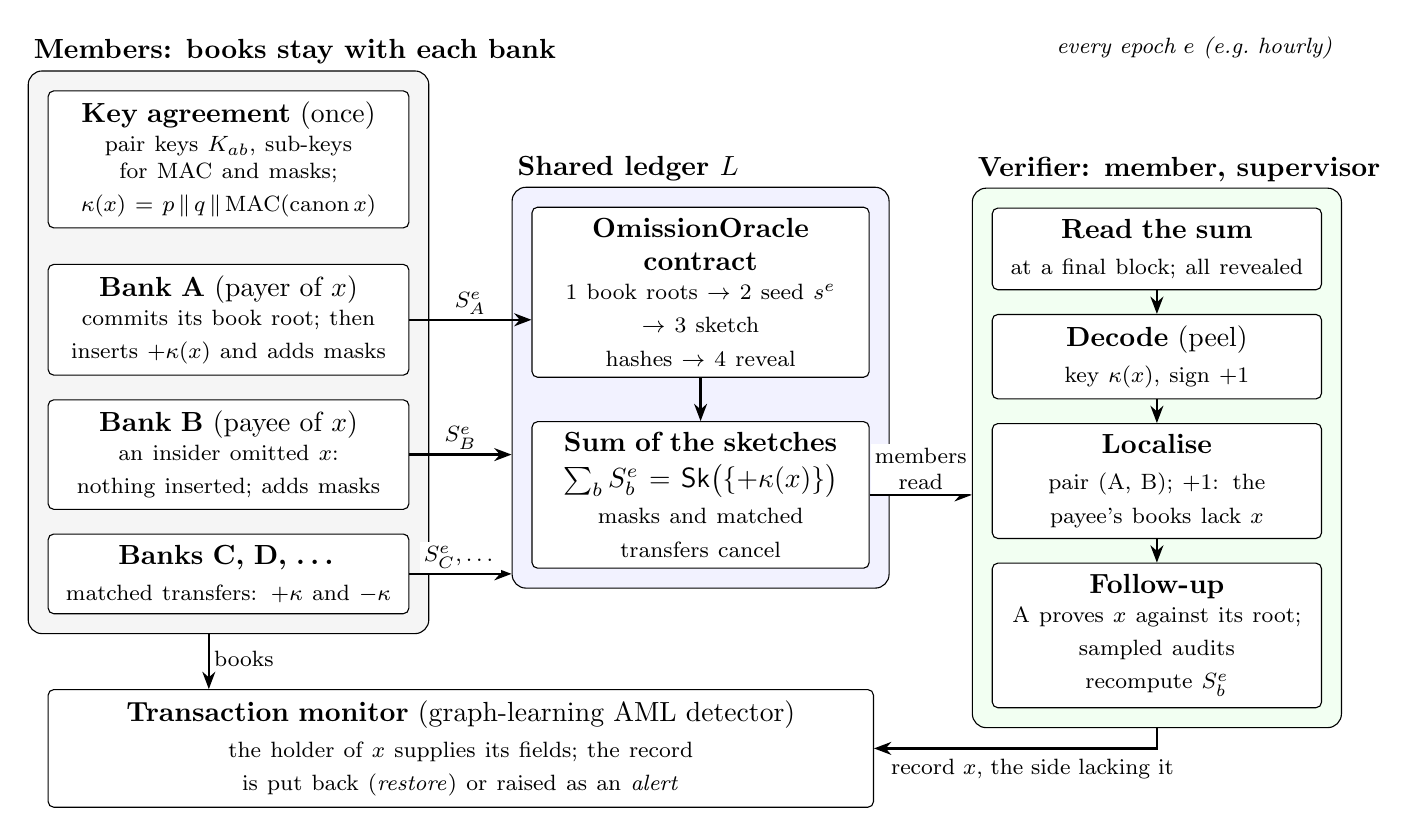
\begin{tikzpicture}[
  font=\normalsize,
  box/.style={draw, rounded corners=2pt, align=center, inner sep=4pt, fill=white, text width=#1,
    execute at begin node={\hyphenpenalty=10000\exhyphenpenalty=10000}},
  box/.default=4.3cm,
  grp/.style={draw, rounded corners=5pt, inner sep=7pt},
  title/.style={font=\normalsize\bfseries, anchor=south west, inner sep=2pt},
  arr/.style={-{Stealth[length=2.2mm]}, thick},
  lbl/.style={font=\footnotesize, fill=white, inner sep=1.5pt, align=center},
]
% ------------------------------------------------------------------ consortium members
\node[box] (keys) at (0,0) {\textbf{Key agreement} (once)\\[1pt]
  \footnotesize pair keys $K_{ab}$, sub-keys for MAC and masks;\\ $\kappa(x)=p\,\|\,q\,\|\,\mathrm{MAC}(\mathrm{canon}\,x)$};
\node[box, below=0.45cm of keys] (A) {\textbf{Bank A} (payer of $x$)\\[1pt]
  \footnotesize commits its book root; then\\ inserts $+\kappa(x)$ and adds masks};
\node[box, below=0.3cm of A] (B) {\textbf{Bank B} (payee of $x$)\\[1pt]
  \footnotesize an insider omitted $x$:\\ nothing inserted; adds masks};
\node[box, below=0.3cm of B] (C) {\textbf{Banks C, D, \dots}\\[1pt]
  \footnotesize matched transfers: $+\kappa$ and $-\kappa$};
\begin{scope}[on background layer]
  \node[grp, fill=black!4, fit=(keys)(A)(B)(C)] (banks) {};
\end{scope}
\node[title] at (banks.north west) {Members: books stay with each bank};

% ------------------------------------------------------------------ ledger
\node[box=4.0cm, right=1.55cm of A.east, anchor=west, yshift=0.35cm] (oracle) {\textbf{OmissionOracle contract}\\[1pt]
  \footnotesize 1 book roots $\to$ 2 seed $s^e$\\ $\to$ 3 sketch hashes $\to$ 4 reveal};
\node[box=4.0cm, below=0.55cm of oracle] (sum) {\textbf{Sum of the sketches}\\[1pt]
  $\sum_b S_b^e=\Sk\big(\{+\kappa(x)\}\big)$\\[1pt]
  \footnotesize masks and matched transfers cancel};
\begin{scope}[on background layer]
  \node[grp, fill=blue!5, fit=(oracle)(sum)] (ledger) {};
\end{scope}
\node[title, align=left] at (ledger.north west) {Shared ledger $L$};

% ------------------------------------------------------------------ verifier
\node[box=3.9cm, right=1.55cm of oracle.east, anchor=west, yshift=0.55cm] (read) {\textbf{Read the sum}\\[1pt]
  \footnotesize at a final block; all revealed};
\node[box=3.9cm, below=0.3cm of read] (peel) {\textbf{Decode} (peel)\\[1pt]
  \footnotesize key $\kappa(x)$, sign $+1$};
\node[box=3.9cm, below=0.3cm of peel] (attr) {\textbf{Localise}\\[1pt]
  \footnotesize pair (A, B); $+1$: the payee's books lack $x$};
\node[box=3.9cm, below=0.3cm of attr] (audit) {\textbf{Follow-up}\\[1pt]
  \footnotesize A proves $x$ against its root;\\ sampled audits recompute $S_b^e$};
\begin{scope}[on background layer]
  \node[grp, fill=green!5, fit=(read)(peel)(attr)(audit)] (verif) {};
\end{scope}
\node[title] at (verif.north west) {Verifier: member, supervisor};
\draw[arr] (read) -- (peel); \draw[arr] (peel) -- (attr); \draw[arr] (attr) -- (audit);

% ------------------------------------------------------------------ AML monitor
\node[box=10.2cm, below=0.95cm of C.south west, anchor=north west] (aml) {\textbf{Transaction monitor} (graph-learning AML detector)\\[1pt]
  \footnotesize the holder of $x$ supplies its fields; the record is put back (\emph{restore}) or raised as an \emph{alert}};

% ------------------------------------------------------------------ flows
\draw[arr] (A.east) -- node[lbl, above, pos=0.5] {$S_A^e$} (oracle.west |- A.east);
\draw[arr] (B.east) -- node[lbl, above, pos=0.5] {$S_B^e$} (ledger.west |- B.east);
\draw[arr] (C.east) -- node[lbl, above, pos=0.5] {$S_C^e,\dots$} (ledger.west |- C.east);
\draw[arr] (oracle) -- (sum);
\draw[arr] (sum.east) -- node[lbl, above] {members\\read} (sum.east -| verif.west);
\draw[arr] (banks.south -| aml.north) ++(-3.2,0) coordinate (bk) -- (bk |- aml.north) node[lbl, pos=0.45, right] {books};
\draw[arr] (verif.south) |- node[lbl, pos=0.72, below=2pt] {record $x$, the side lacking it} (aml.east);
\node[font=\footnotesize\itshape, anchor=north east] at (verif.north east |- banks.north) [yshift=0.55cm] {every epoch $e$ (e.g.\ hourly)};
\end{tikzpicture}
\end{document}
